\clearpage
\section{Service Equipment and Incense}
Processional and service articles---cross, candles, cruets, lavabo, bells, holy water, and incense---give visible, audible, and fragrant reverence to the entrance of Christ's ministers, the proclamation of the Gospel, the offering of the gifts, and the consecration of the Eucharist.

\PCDPlateHeader{Plate VI --- Processional and Service Equipment}{Not to common scale}
\ifdefined\TriptychPrintEdition
\begin{center}
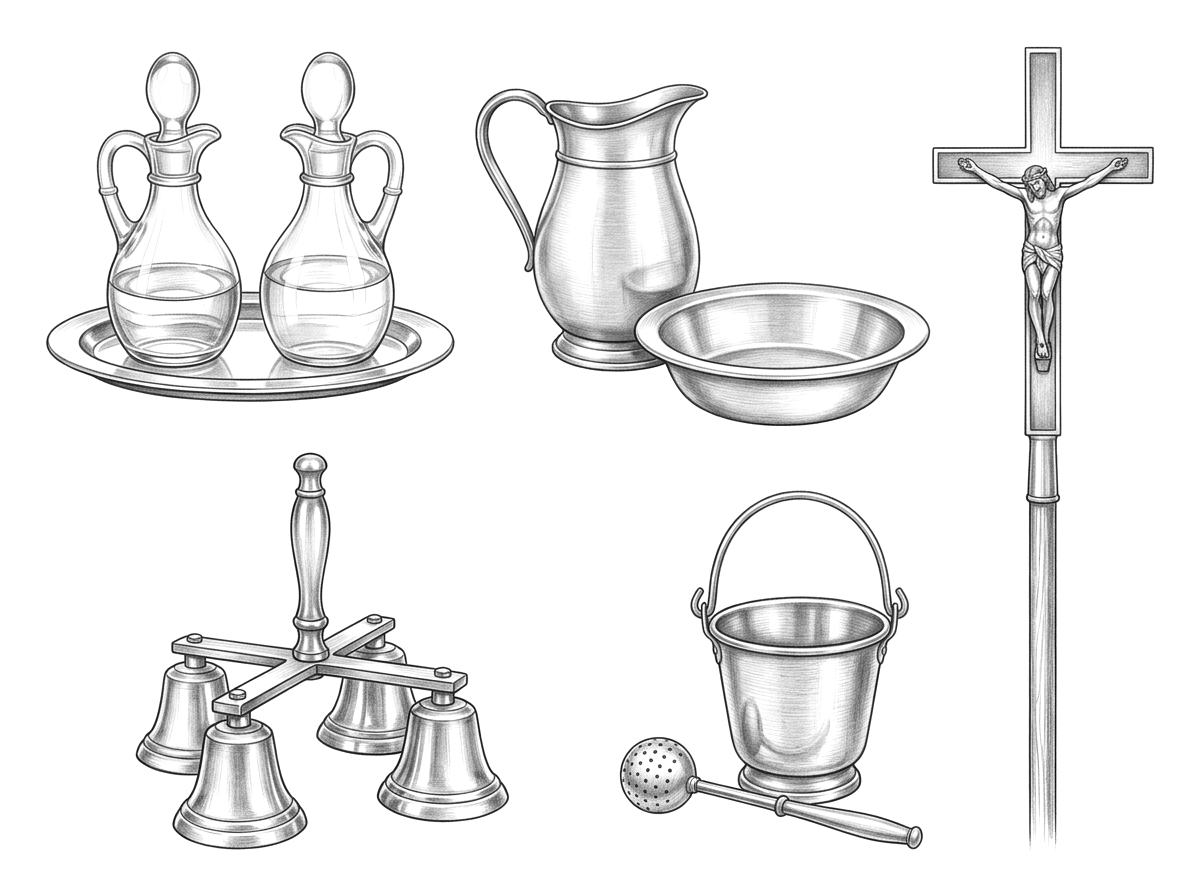
\includegraphics[width=0.92\linewidth,height=3.55in,keepaspectratio]{liturgy/roman-rite/postconciliar/2008-latin-2011-us-english/reference/roman-sanctuary-dictionary/shared/artwork/graphite/pc-art-06-service-cruets-bells.png}
\end{center}
\PCDPositionKey{Top left: paired glass wine and water Cruets with stoppers on a tray; top center: Lavabo pitcher and shallow finger basin; top right: Processional Cross bearing the sculpted corpus of Christ on a staff; bottom left: four-cup mounted brass Sanctuary Bell; bottom right: holy-water Aspersorium bucket and perforated metal Aspergillum.}
\else
\textbf{Visual Plate Summary (Plate VI --- Processional and Service Equipment, Not to common scale):} Five-object monochrome graphite service equipment study: top left, two stoppered transparent glass cruets for wine and water resting on an oval metal tray; top center, a metal lavabo pitcher beside a shallow round finger basin; top right, a tall processional cross on a wooden staff bearing the sculpted figure of Christ crucified; bottom left, a traditional four-bell mounted brass sanctuary hand bell; bottom right, a metal holy-water aspersorium bucket with bail handle and perforated spherical-head aspergillum resting beside it.

\textbf{Reading order and object placement:} Top left: paired glass wine and water Cruets with stoppers on a tray; top center: Lavabo pitcher and shallow finger basin; top right: Processional Cross bearing the sculpted corpus of Christ on a staff; bottom left: four-cup mounted brass Sanctuary Bell; bottom right: holy-water Aspersorium bucket and perforated metal Aspergillum.
\fi

\label{pc-obj-processional-cross}
\PCDEntryHead{Processional Cross}{Crux processionalis}{required}{N25}
\PCDField{Also called}{Altar Cross; Crucifix; \textit{Crux cum figura Christi crucifixi}}
The processional cross is a tall staff-mounted crucifix carried at the head of liturgical processions and often stationed beside the altar to serve as the single altar cross during Mass. A Latin cross bearing the sculpted figure of Christ crucified is fitted into a ringed socket atop a slender cylindrical wooden or metal staff, matching the standing altar crucifix shown at the center of the mensa in Plate I.

\PCDField{Plate position and status}{Top right, bearing sculpted corpus on wooden staff (Plate VI); altar cross at center (Plate I) (Universal Roman law)}
\PCDField{Placement and liturgical use}{During the entrance procession, an instituted acolyte or altar server carries the processional cross between two ministers bearing lighted candles (GIRM 120b). On reaching the sanctuary, the cross may be set in a floor stand near the altar to serve as the altar cross, in which case it must be the only cross present; otherwise it is placed away in a dignified spot while a separate crucifix remains clearly visible on or near the altar (GIRM 117, 122, 308). It is fitting that the cross with the figure of Christ crucified remain near the altar even outside liturgical celebrations (GIRM 308).}
\PCDField{Ministers and server boundary}{Ordinary ministers: Instituted acolyte, Altar server. Server carries in procession or movement: The cross-bearer carries the processional cross upright with the figure of Christ facing forward, omits bowing and genuflecting while holding it (GIRM 274), and sets it securely in its floor stand near the altar or puts it away if another altar cross already stands there (GIRM 122).}
\PCDSafety{Do not bow or genuflect while holding the processional cross (GIRM 274), both to honor the rubric and to prevent the tall staff from pitching forward. Keep the staff clear of low doorways and hanging lights, and confirm that its weighted floor stand is level and stable before releasing it.}
\PCDField{Symbolism}{The cross adorned with the figure of Christ crucified remains visibly before the assembly during Mass and outside liturgical celebrations so as to recall the saving Passion of the Lord (GIRM 308). St. Paul proclaims, ``But we preach Christ crucified'' (1 Cor 1:23) and ``But God forbid that I should glory, save in the cross of our Lord Jesus Christ'' (Gal 6:14), through whom God reconciles all things, ``making peace through the blood of his cross'' (Col 1:20). St. Thomas Aquinas affirms that the consecration of the Eucharist, the acceptance of the sacrifice, and all its fruits flow from the virtue of the Cross of Christ. (GIRM 308; 1 Cor 1:23; Gal 6:14; Col 1:20; St. Thomas Aquinas, Summa Theologiae III, q. 83, a. 5, ad 3)}
\PCDField{1962 Roman Missal counterpart}{\PCDTag{changed use} Whereas the 1962 Roman Missal required a separate crucifix standing in the center of the altar (RG 527) and did not ordinarily prescribe a carried cross at a priest's High Mass entrance, the 2002/2008 GIRM assigns the processional cross with the figure of Christ crucified a regular place in the entrance procession (GIRM 120b) and permits it to stand near the altar as the sole altar cross (GIRM 122, 308). The 2002 third typical edition also restored the explicit requirement of the sculpted corpus that had been omitted in the 1970 and 1975 editions.}
\PCDEntryRule

\label{pc-obj-altar-candles}
\PCDEntryHead{Altar Candles}{Candelabra cum cereis}{required}{N26}
\PCDField{Also called}{Altar Candlesticks; Processional Candles; \textit{Cerei}; \textit{Candelabra}}
Altar candles are lighted wax or oil candles mounted in dignified candlesticks on or around the altar for every liturgical celebration, as well as paired candlesticks carried in processions. Two slender footed candlesticks bearing tall white wax tapers flank the central crucifix on the freestanding altar in Plate I, each fitted with a shallow wax bobeche to catch melted drips.

\PCDField{Plate position and status}{See Plate I, flanking the freestanding altar (Universal Roman law)}
\PCDField{Placement and liturgical use}{At every celebration of Mass, lighted candles are placed on or around the altar: at least two candlesticks, or four or six especially for Sunday Mass and Holy Days of Obligation, and seven when the Diocesan Bishop celebrates (GIRM 117). Candlesticks are arranged harmoniously with the architecture of the altar and sanctuary so that they never obstruct the assembly's clear view of what takes place upon the mensa (GIRM 307). Two lighted candles also accompany the processional cross at the entrance procession and flank the Book of the Gospels during the Gospel procession and proclamation at the ambo (GIRM 120b, 133, 175).}
\PCDField{United States norm}{GIRM 117 and 307 are universal Roman norms without a separate territorial insertion for the United States. Guidance of the USCCB Committee on Divine Worship maintains real living flames of wax or oil rather than electric lights.}
\PCDField{Ministers and server boundary}{Ordinary ministers: Instituted acolyte, Altar server. Server handles directly: Servers light altar candles shortly before Mass, extinguish them cleanly with a snuffer afterward, and carry processional and Gospel candles upright at matching heights without bowing or genuflecting while holding them (GIRM 120b, 133, 274).}
\PCDSafety{Keep open flames well clear of hair, albs, ribbons, vestments, and the pages of the Roman Missal. Carry processional candles strictly upright, watch for dripping hot wax, and extinguish every flame with a brass snuffer rather than blowing melted wax onto the white altar cloth.}
\PCDField{Distinguish from}{Sanctuary Lamp}
\PCDField{Symbolism}{Candles are lighted at every liturgical celebration to express reverence and festive honor before God (GIRM 117, 307). Their living flame recalls Christ, who declares in the Gospel, ``I am the light of the world. He that followeth me walketh not in darkness, but shall have the light of life'' (John 8:12). (GIRM 117, 307; John 8:12)}
\PCDField{1962 Roman Missal counterpart}{\PCDTag{materially changed} Both the 1962 Roman Missal (RG 527) and the 2002/2008 GIRM (117, 307) scale candle counts from two up to six, or seven for the Diocesan Bishop. In 1962, altar candlesticks stood directly on the altar or its gradine flanking the central crucifix, supplemented by separate Sanctus and elevation torches; postconciliar GIRM 117, 122, and 307 permit candlesticks to stand either on or around the altar---including processional candlesticks placed near it---so that the faithful maintain an unobstructed view of the altar table.}
\PCDEntryRule

\label{pc-obj-sanctuary-bells}
\PCDEntryHead{Sanctuary Bells}{Campanula}{optional}{N27}
\PCDField{Also called}{Altar Bell; Sanctus Bell; \textit{Parva campanula}}
Sanctuary bells are a small hand bell or multi-cup brass chime rung optionally by a server during the Eucharistic Prayer to alert the congregation to the consecration. Four tuned, flared brass bell cups hang from the arms of a horizontal cruciform yoke topped by a central turned vertical handle, though single hand bells and three-cup sets are also common.

\PCDField{Plate position and status}{Bottom left, four-cup mounted brass altar bell (Plate VI) (Documented custom)}
\PCDField{Placement and liturgical use}{When used according to local custom, the sanctuary bell rests on the credence table or beside the servers' kneeling place before the Eucharistic Prayer. Shortly before the consecration---customarily as the priest extends his hands over the gifts at the epiclesis---an instituted acolyte or altar server may give a crisp signal on the bell, and likewise ring it at each showing of the consecrated Host and Chalice (GIRM 150). Bells remain silent from the conclusion of the Gloria at the Evening Mass of the Lord's Supper on Holy Thursday until the Gloria of the Easter Vigil.}
\PCDField{Ministers and server boundary}{Ordinary ministers: Altar server, Instituted acolyte. Server handles directly: An altar server rings the sanctuary bell cleanly and reverently shortly before the consecration and at each elevation according to local parish custom (GIRM 150), setting it down quietly without rattling the cups.}
\PCDField{1962 Roman Missal counterpart}{\PCDTag{optional} Whereas the 1962 Roman Missal required a small bell on the Epistle-side table and prescribed ringing at the Sanctus and elevations (RG 528; RS VII.8, VIII.6), the 2002/2008 GIRM makes the bell optional according to local custom---shortly before the consecration and at each showing of the Host and Chalice---omitting the mandatory Sanctus and Communion rings (GIRM 150).}
\PCDEntryRule

\label{pc-obj-aspergillum-aspersorium}
\PCDEntryHead{Aspergillum and Aspersorium}{Aspergillum et aspersorium}{optional}{N28}
\PCDField{Also called}{Holy-Water Sprinkler and Bucket; Holy-Water Vessel; \textit{Vas aquae benedicendae}; \textit{Vas aquae benedictae}}
The aspersorium is the portable vessel that holds blessed water, paired with the aspergillum, the handheld sprinkler used to cast holy water over the assembly, altar, or blessed objects. A tapered cylindrical metal bucket rests on a molded circular foot with an arched wire bail handle hooked to twin rim lugs; beside it lies a turned metal sprinkler handle ending in a perforated hollow sphere (some parishes also use a bristled brush or natural evergreen branch).

\PCDField{Plate position and status}{Bottom right, holy-water bucket and perforated sprinkler (Plate VI) (Universal Roman law)}
\PCDField{Placement and liturgical use}{On Sundays, especially during Easter Time, the Order for the Blessing and Sprinkling of Water may replace the ordinary Penitential Act within the Introductory Rites of Mass (GIRM 51; Roman Missal, Appendix II). When the sprinkling rite is scheduled, the clean vessel of water to be blessed (or already blessed, as at the Easter Vigil) is prepared with the sprinkler on the credence table (GIRM 118c). The priest---vested in his chasuble---blesses the water, sprinkles himself and the ministers, and walks through the church sprinkling the faithful while a deacon or server carries the bucket beside him. The same paired instruments serve at funerals, church blessings, and sacramentals in the Book of Blessings.}
\PCDField{Ministers and server boundary}{Ordinary ministers: Bishop, Priest, Deacon. Server carries and presents to priest or deacon: Servers fill the clean vessel on the credence table before Mass, bring it to the priest for the blessing and sprinkling rite, accompany him through the nave holding the bucket steady, and return both articles cleanly to the credence table afterward (GIRM 51, 118c).}
\PCDSafety{Fill the bucket only half to two-thirds full so water does not slosh over the rim onto stone or polished sanctuary steps and create a slipping hazard for ministers and communicants.}
\PCDField{Distinguish from}{Cruets, Baptismal Font}
\PCDField{Symbolism}{The bucket and sprinkler are practical service instruments; the sacred symbolism belongs to the sprinkling rite itself, which recalls the grace and cleansing of Baptism (GIRM 51; Roman Missal, Appendix II). Its classic antiphon echoes the Psalmist: ``Thou shalt sprinkle me with hyssop, and I shall be cleansed: thou shalt wash me, and I shall be made whiter than snow'' (Ps 50:9 [Heb 51:7]). (GIRM 51; Roman Missal, Appendix II; Ps 50:9 [Heb 51:7])}
\PCDField{1962 Roman Missal counterpart}{\PCDTag{changed use} Although the portable metal bucket and sprinkler continue unchanged in form, the 1962 Roman Missal placed the Sunday Asperges me or Vidi aquam before the start of Mass, with the water blessed in the sacristy and the celebrant wearing a cope before putting on the chasuble. In the 2002/2008 Roman Missal, the Blessing and Sprinkling of Water takes place inside the Introductory Rites in place of the Penitential Act, celebrated by the priest already vested in his chasuble (GIRM 51, 118c; Appendix II).}
\PCDEntryRule

\clearpage
\subsection{Incense Equipment}
\PCDPlateHeader{Plate VII --- Incense Equipment}{Not to common scale}
\ifdefined\TriptychPrintEdition
\begin{center}
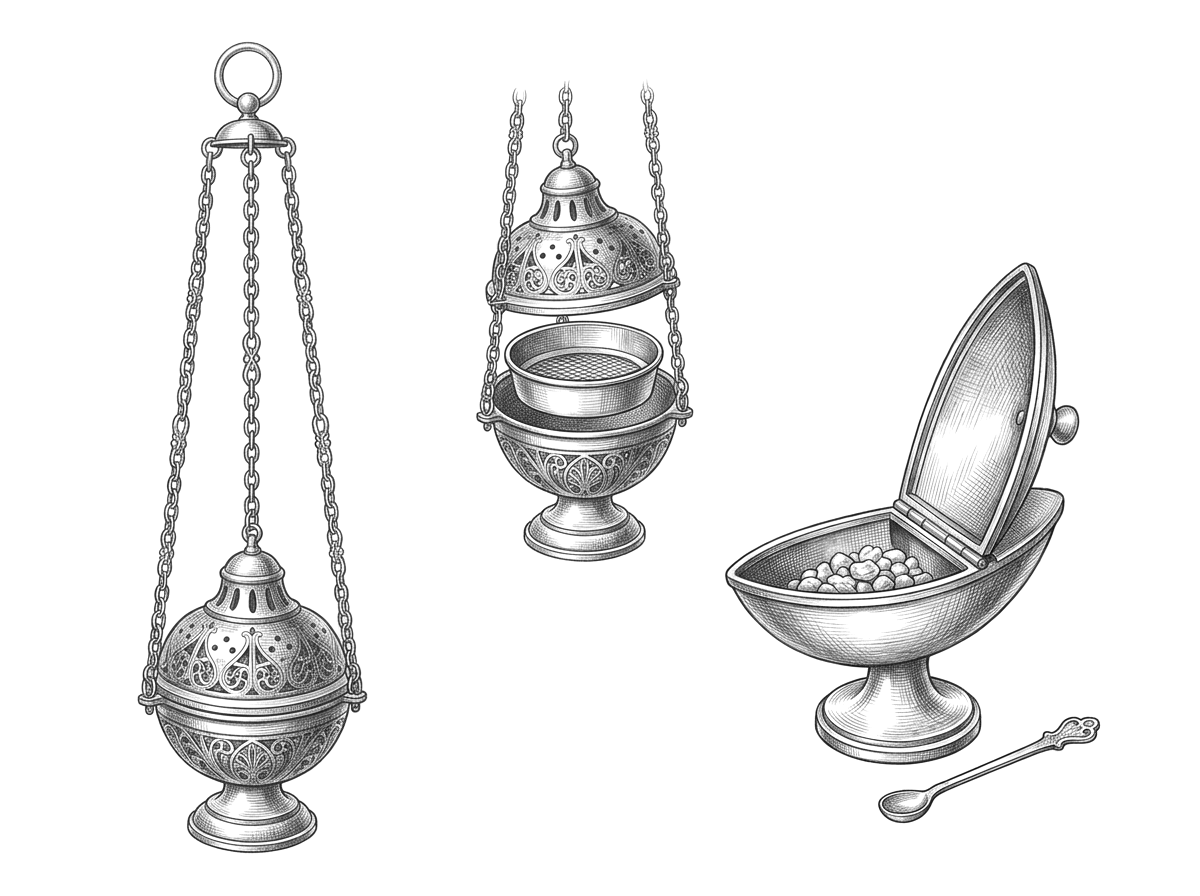
\includegraphics[width=0.92\linewidth,height=3.55in,keepaspectratio]{liturgy/roman-rite/postconciliar/2008-latin-2011-us-english/reference/roman-sanctuary-dictionary/shared/artwork/graphite/pc-art-07-incense-set.png}
\end{center}
\PCDPositionKey{Left: closed metal Thurible suspended on outer rim chains (two visible in profile) and one central lid-lifting chain; center: detail of raised perforated dome revealing removable inner charcoal fire-pan; right: footed Incense Boat (navicula) with hinged half-lid open showing resin grains, accompanied by its metal spoon.}
\else
\textbf{Visual Plate Summary (Plate VII --- Incense Equipment, Not to common scale):} Three-part monochrome graphite incense study: left, a classical footed metal thurible hanging vertically from its top ring on outer rim chains (two visible in profile) and a central lid-lifting chain with perforated domed cover closed; center, a sectional open view with the dome lifted to expose the removable circular charcoal fire-pan; right, a pedestal-footed boat-shaped incense boat with hinged half-lid open showing resin incense grains, paired with a small long-handled metal spoon.

\textbf{Reading order and object placement:} Left: closed metal Thurible suspended on outer rim chains (two visible in profile) and one central lid-lifting chain; center: detail of raised perforated dome revealing removable inner charcoal fire-pan; right: footed Incense Boat (navicula) with hinged half-lid open showing resin grains, accompanied by its metal spoon.
\fi

\label{pc-obj-thurible}
\PCDEntryHead{Thurible}{Turibulum}{optional}{N29}
\PCDField{Also called}{Censer; \textit{Thuribulum}}
The thurible is a chained metal censer in which fragrant resin incense is burned upon glowing charcoal during Mass, Eucharistic Benediction, solemn Liturgy of the Hours, and funerals. A footed metal bowl decorated in relief hangs from a top finger ring on outer rim chains (two visible in profile on Plate VII), while a central chain lifts the perforated domed cover to expose the removable circular charcoal fire-pan and grate shown in the center detail of Plate VII.

\PCDField{Plate position and status}{Left (closed on chains) and center inset (dome lifted revealing inner charcoal fire-pan) (Plate VII) (Universal Roman law)}
\PCDField{Placement and liturgical use}{Incense may be used optionally in any form of Mass at five appointed moments: during the entrance procession, at the start of Mass to incense the cross and altar, at the Gospel procession and proclamation, after the bread and chalice are placed on the altar to incense the offerings, cross, altar, priest, and people, and at the showing of the Host and Chalice after the consecration (GIRM 120a, 133, 144, 150, 276). The priest imposes incense onto the charcoal and blesses it silently with the Sign of the Cross (GIRM 277). Incensation follows the rhythmic swing pattern of GIRM 277---three swings (tribus ductibus) for the Blessed Sacrament, a relic of the True Cross, images of the Lord, the offerings, the altar cross, the Book of the Gospels, the paschal candle, the priest, and the people; two swings (duobus ductibus) for relics and images of the Saints; and continuous single swings while walking around the altar (each ductus being executed as a paired double swing in Roman ceremonial custom, Caeremoniale Episcoporum 92)---framed by a profound bow before and after except when incensing the altar and offerings.}
\PCDField{Ministers and server boundary}{Ordinary ministers: Bishop, Priest, Deacon, Instituted acolyte, Altar server. Server handles directly: The thurifer lights charcoal safely in the sacristy, leads the entrance procession with the smoking thurible, raises the dome steadily for the priest to impose incense, hands the censer to the priest or deacon, and---when no deacon serves---incenses the priest, assembly, and consecrated Host and Chalice at the elevations (GIRM 120a, 150, 277).}
\PCDSafety{Handle burning charcoal exclusively with metal tongs, never with bare fingers. Keep the hot bowl and chains clear of vestments, white altar linens, and narrow aisles, swing only with controlled short wrist movements, and empty spent coals into a dedicated fireproof metal ash vessel rather than an ordinary trash bin.}
\PCDField{Distinguish from}{Sanctuary Lamp}
\PCDField{Symbolism}{Incensation expresses reverence and rising prayer before God (GIRM 276), grounded directly in Sacred Scripture: ``Let my prayer be directed as incense in thy sight; the lifting up of my hands, as evening sacrifice'' (Ps 140:2 [Heb 141:2]), and in the heavenly liturgy of the Apocalypse, ``And the smoke of the incense of the prayers of the saints ascended up before God from the hand of the angel'' (Apoc 8:4; cf. Apoc 5:8, 8:3). St. Thomas Aquinas adds that the fragrant smoke signifies the grace of Christ spreading through His ministers, echoing St. Paul's words that God ``manifesteth the odour of his knowledge by us in every place'' (2 Cor 2:14). (GIRM 276; Ps 140:2 [Heb 141:2]; Apoc 5:8, 8:3--4; 2 Cor 2:14; St. Thomas Aquinas, Summa Theologiae III, q. 83, a. 5, ad 2)}
\PCDField{1962 Roman Missal counterpart}{\PCDTag{changed use} In the 1962 Roman Missal, incense at Mass was restricted to Solemn Mass and permitted sung Masses (never Low Mass) and accompanied by spoken blessing and incensation prayers (Ordo Missae 1035--1038). The 2002/2008 GIRM permits incense optionally in any form of Mass at five enumerated moments, replaces the spoken blessing with a silent Sign of the Cross, and codifies standardized sets of three, two, and single swings (GIRM 276--277).}
\PCDEntryRule

\label{pc-obj-incense-boat}
\PCDEntryHead{Incense Boat}{Navicula}{optional}{N30}
\PCDField{Also called}{Incense Boat and Spoon; \textit{Navicula cum cochleari}}
The incense boat is a small lidded metal container with a companion spoon used to hold unburned resin incense grains and transfer them onto the glowing charcoal of the thurible. Shaped like a miniature hull resting on a flared pedestal foot, the vessel features a hinged half-lid lifted by a side knob to reveal granular resin incense inside, accompanied by a slender long-handled metal spoon resting beside its base.

\PCDField{Plate position and status}{Right, boat-shaped vessel with hinged half-lid open and spoon beside base (Plate VII) (Universal Roman law)}
\PCDField{Placement and liturgical use}{Whenever incense is employed during Mass, Benediction, or solemn Liturgy of the Hours (GIRM 120, 276--277), the incense boat accompanies the thurible. A dedicated boat-bearer---or the thurifer holding the boat in the left hand when serving alone---presents the opened vessel to the priest or deacon so that the priest may spoon resin grains onto the hot coals and bless them silently with the Sign of the Cross (GIRM 277).}
\PCDField{Ministers and server boundary}{Ordinary ministers: Priest, Deacon, Instituted acolyte, Altar server. Server carries and presents to priest or deacon: The boat-bearer (or lone thurifer) opens the hinged lid and offers the spoon handle toward the priest or deacon before each imposition of incense, closing the lid promptly before walking so resin grains do not spill on sanctuary steps (GIRM 277).}
\PCDField{1962 Roman Missal counterpart}{\PCDTag{continued} Both the 1962 Roman Missal (RS IV.4, VII.10) and the 2002/2008 GIRM (120, 276--277) pair the incense boat and spoon with the thurible. In postconciliar practice, the priest imposes incense silently with a Sign of the Cross rather than speaking the 1962 blessing formula, and neither the spoon nor the celebrant's hand is kissed at the presentation.}
\PCDEntryRule
